\documentclass[11pt]{article}
\usepackage[margin=1in]{geometry}
\usepackage{amsmath,amssymb,booktabs,graphicx,setspace,caption,hyperref}
\usepackage[T1]{fontenc}
\usepackage{mathpazo}
\setlength{\parindent}{0pt}
\setlength{\parskip}{0.6em}
\captionsetup{font=small,skip=6pt}
\title{Panel MS-AR(1) for EMBI countries from 1990\\[0.4em]\large Common trend, random intercepts, and catch-up}
\author{}
\date{}
\begin{document}
\maketitle
\section{Model}
All countries in the 2026-09-17 panel that are in the J.P.\ Morgan EMBI Global as of April 2025, or on an earlier published EMBI Global list (Korea, Thailand, Croatia, and Tunisia). No country is dropped. The sample starts in 1990.
Step 1 builds a common trend from average growth of countries observed in consecutive quarters:
\begin{align}
\Delta\tau_t &= \frac{1}{n_t^{\mathrm{cont}}}\sum_{i\in C_t\cap C_{t-1}}(y_{it}-y_{i,t-1}), \\
\tau_t &= \tau_{t_0}+\sum_{s=t_0+1}^{t}\Delta\tau_s.
\end{align}
Mean $\Delta\tau$ is 0.0047 per quarter (1 countries present every quarter). The level of $\tau$ is an arbitrary pin; a common shift is absorbed by $\alpha$. Step 2 uses $y_{it}^\ast=y_{it}-\hat\tau_t$:
\begin{align}
y_{it}^\ast &= a_i + b_i\lambda^{t-T_{i0}} + z_{it}, \\
a_i &\sim \mathcal{N}(\alpha,\omega^2),\qquad b_i \sim \mathcal{N}(0,\omega_b^2)\ \text{independent}, \\
z_{i,t+1} &= \bigl(1-\rho(s_{it})\bigr)\mu(s_{it}) + \rho(s_{it})\, z_{it} + \sigma(s_{it})\,\varepsilon_{it}.
\end{align}
$\lambda=0.98$ is fixed (Barro, about 2\% per year). $T_{i0}$ is country $i$'s first observation in this sample. Three regimes. $E[z]=0$. $\sigma$ and $\rho$ switch, $|\rho|<0.99$. Random effects use a $7\times 7$ Gauss--Hermite grid. Standard errors ignore step-1 uncertainty.
\begin{figure}[h]
\centering
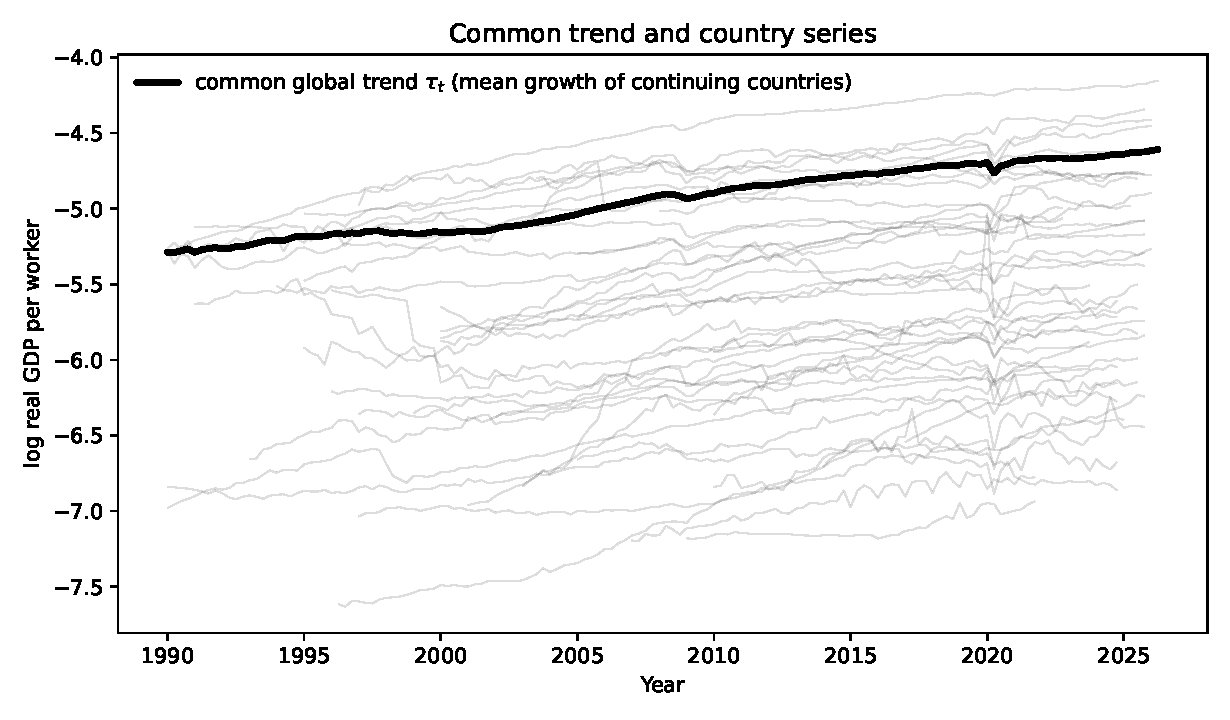
\includegraphics[width=0.88\textwidth]{figs/tau_embi_1990_barro.pdf}
\caption{Faint lines: country log real GDP per worker. Thick line: common $\tau_t$.}
\end{figure}
\clearpage
\section{EMBI from 1990: common RW trend, RE intercepts, Barro catch-up}
EMBI countries, 1990 onward, $y_{it}=a_i+\tau_t+b_i\lambda^{t-T_{i0}}+z_{it}$, $\lambda=0.98$, $E[z]=0$. 43 countries, 4275 observations, 1990-Q1--2026-Q2. Fitted countries: 43. Observations: 4275. Log-likelihood: 10571.80.
Permanent RE intercepts and catch-up $y_{it}=a_i + b_i\lambda^{t-T_{i0}}+z_{it}$ with $\alpha=-1.1949$ (0.0273), $\omega=0.7032$ (0.0139), $\lambda=0.9800$ (fixed), $\omega_b=0.4799$ (0.0242). Posterior-mean $a_i$: mean -0.930, min -2.858, max 0.469. Posterior-mean $b_i$: mean 0.056, min -1.224, max 1.136.
\begin{table}[h]
\centering
\caption{Regime AR(1), transition matrix, and ergodic $\pi$. Columns are regimes.}
\begin{tabular}{lccc}
\toprule
 & (0) & (1) & (2) \\
\midrule
$\mu$ & -0.0845 & -0.0161 & 0.1099 \\
 & (0.0413) & --- & (0.0264) \\ \addlinespace
$\sigma$ & 0.0243 & 0.0892 & 0.0095 \\
 & (0.0010) & (0.0055) & (0.0003) \\ \addlinespace
$\rho$ & 0.9900 & 0.7826 & 0.9900 \\
 & (0.0001) & (0.0574) & (0.0001) \\ \addlinespace
$\Pi_{0\cdot}$ & 0.9023 & 0.0320 & 0.0658 \\
 & (0.0136) & (0.0089) & (0.0126) \\ \addlinespace
$\Pi_{1\cdot}$ & 0.3017 & 0.6803 & 0.0180 \\
 & (0.0600) & (0.0575) & (0.0202) \\ \addlinespace
$\Pi_{2\cdot}$ & 0.0594 & 0.0090 & 0.9316 \\
 & (0.0101) & (0.0046) & (0.0094) \\ \addlinespace
$\pi$ & 0.4711 & 0.0603 & 0.4686 \\
 & (0.0328) & (0.0112) & (0.0365) \\ \addlinespace
\bottomrule
\end{tabular}
\end{table}
\begin{figure}[h]
\centering
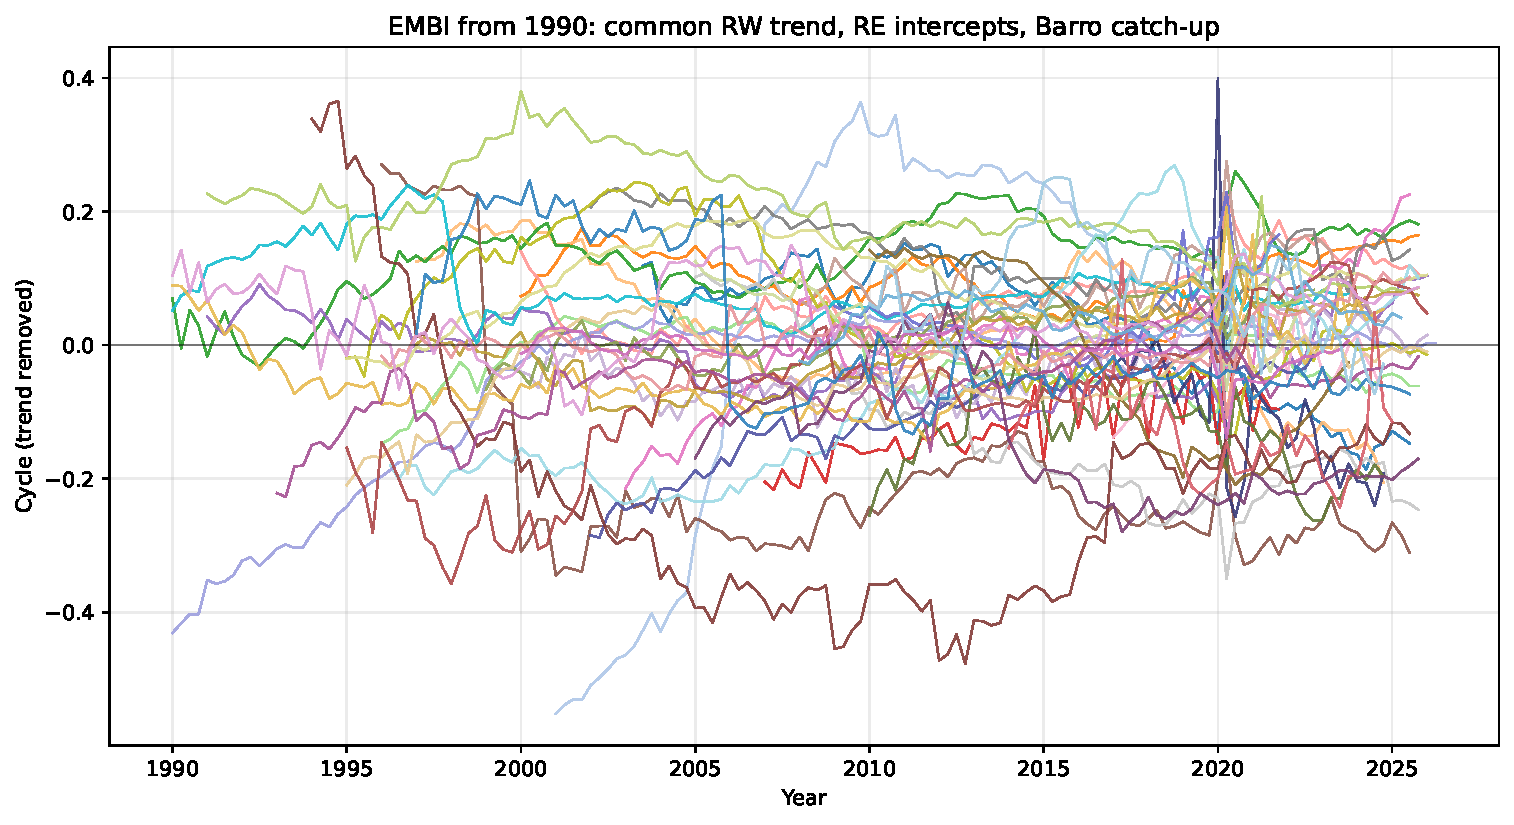
\includegraphics[width=0.75\textwidth]{figs/cycle_embi_1990_rw_barro.pdf}
\caption{Country cycles after removing $\tau_t$, $a_i$, and $b_i\lambda^{t-T_{i0}}$.}
\end{figure}
\end{document}
